\documentclass{beamer}
\usetheme{metropolis} % Use metropolis theme

\renewcommand{\footnoterule}{%
  \hspace{10cm}
  \kern -3pt
  \hrule width \textwidth height 1pt
  \kern 2pt
}
\usepackage[utf8]{inputenc}
\usepackage[T1]{fontenc}
\usepackage[british]{babel}
\usepackage[autostyle, english = british]{csquotes}
\usepackage[%
  backend=biber,
  doi=false,
  url=false,
  isbn=false,
  eprint=false,
  style=authoryear,
  hyperref=true,
  maxnames=9,
  minnames=9,
  maxbibnames=99,
  firstinits,
  uniquename=init]{biblatex}
\addbibresource{../bibliography.bib}

\usepackage{caption}
\usepackage{xpatch}
\usepackage{bm}
\usepackage{amsmath}
\usepackage{mathtools} % for \mathclap
\usepackage{varioref}
\usepackage{booktabs}
\usepackage{siunitx}
\usepackage{hyperref}
\usepackage[noabbrev]{cleveref}
\newcommand{\creflastconjunction}{, and\nobreakspace} % use Oxford comma
\usepackage{todonotes}
\usepackage{phaistos}
\usepackage{multimedia}
\usepackage{tikz}
\usetikzlibrary{arrows, positioning, shapes.geometric}
\usetikzlibrary{calc}
\usepackage{pgfgantt}


\graphicspath{{../../figures/}}

\newcommand{\cn}{\textbf{TODO: Citation}}
\newrobustcmd*{\bftabnum}{%
  \bfseries
  \sisetup{output-decimal-marker={\textmd{.}}}%
}
\sisetup{detect-weight=true,detect-inline-weight=math}

\title{Data-Driven Models for Zebrafish Motion\\IDP final}
\author{Lukas Krenz\\
Advisers: Dr.\ Jacob Davidson (Constance), Nicola Rieke (CAMP)\\
Supervisor: Prof.\ Dr.\ Nassir Navab}
\date{July 1, 2018} 
\institute{TUM, Chair for Computer Aided Medical Procedures \textit{\&} Augmented Reality\\
Collaboration with Couzin Lab (Max Plank Institute for Ornithology/University of Constance)
}

\begin{document}
\maketitle
\begin{frame}{Introduction}
Goal: Develop models for social behavior of juvenile zebrafish that extend to large groups.

Contributions:
\begin{itemize}
\item Comparison of models with increasing complexity for modeling interactions between two fish
\item Data-driven spatial discretization
\item Evaluation of importance of past trajectories
\item Development and evaluation of a non-linear recurrent neural network that predicts parameters for mixture of Gaussians
\end{itemize}

Example \textbf{use case}: controlling a fish in a virtual reality environment\\
``Pilot experiment'' for neural network models for collective motion
\end{frame}

\begin{frame}{Zebrafish: Our Input Video} 
\begin{figure}[H]
    \centering
    \movie[width=0.7\textwidth, height=0.7\textwidth, autostart,, loop, poster]{}{motion_experiment.mp4}
\end{figure}
\end{frame}

\begin{frame}
  \frametitle{Modeling Fish Motion}
Data: Annotated (\alert{no tracking needed}) videos from 10 experiments with 2 fish swimming, each for 1h.
Annotations: positions of both fish and their orientation

Segmentation into c.a.\ 148000 kicks

Use wall model\footfullcite{calovi} to ignore areas with high wall influence (any wall closer than c.a.\ \SI{4.8}{\cm}).

Final data: c.a.\ 19400 kicks in training set (80\% of all kicks)

We \alert{model} kick trajectory (=kick direction and kick length).
\end{frame}

\begin{frame}
  \frametitle{Receptive Field\footfullcite{discreteModes}---Local coordinate system}
  \begin{columns}
   \begin{column}{0.5\textwidth}
     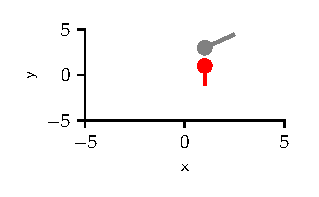
\includegraphics{receptive_field_before_beamer}
\end{column}~\begin{column}{0.5\textwidth}
     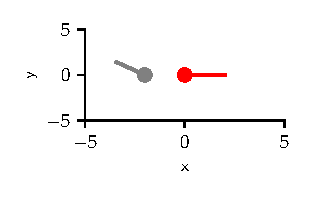
\includegraphics{receptive_field_after_beamer}
\end{column}
 \end{columns}
 
 Rotate coordinate system s.t.\ focal fish (red) has angle 0 (parallel to x-axis) and is at origin.
\end{frame}

\begin{frame}
  \frametitle{Receptive Field---Discretization}
  We discretize the area surrounding the fish in the local coordinate system.

  We want:
  \begin{itemize}
  \item Symmetry around origin: to distinguish left/right, before/behind
  \item Bins should have equal number of fish.
  \end{itemize}

  Use $8 \times 8$ bins.
  
  Discretizing (with symmetry) axes independently is standard approach.
  
  \textbf{But}:
  mean number of data points per bin of roughly \(2428\pm 8483\) (mean $\pm$ std.) for training and
  \(555 \pm 1926\) for testing.

12 bins \alert{completely empty}, even for \textbf{training set}!
\end{frame}

\begin{frame}
  \frametitle{Receptive Field---Data-driven discretization}
  \begin{figure}
    \centering
  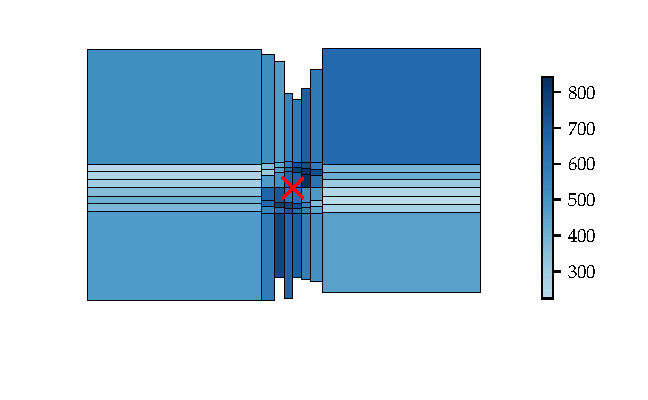
\includegraphics{rf_occupancy_test_beamer}
  \caption*{Mean number of kicks per testing bin}
  \end{figure}
  \vspace{-0.5cm}
Leads to  $2482 \pm 212$ and $555 \pm 162$ data points per bin, instead of \(2428\pm 8483\) and \(555 \pm 1926\).
\end{frame}

\begin{frame}
  \frametitle{Receptive Field---Data-driven discretization (zoomed in)}
  \begin{figure}
  \centering
  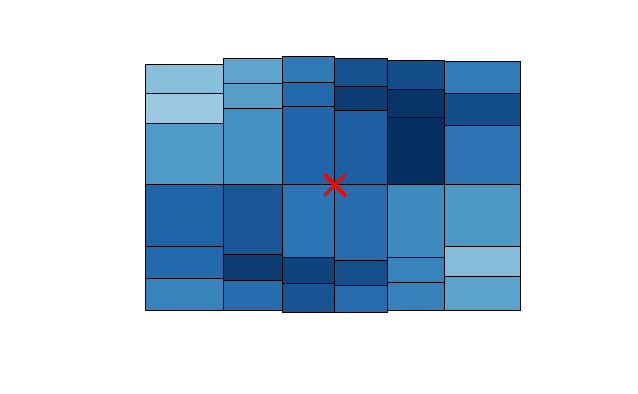
\includegraphics{rf_occupancy_test_zoomed_beamer}

   \caption*{Mean number of kicks per testing bin}
 \end{figure}
\end{frame}

\begin{frame}
  \frametitle{Receptive Field---Extracted features}
  Bin number is one-hot encoded, alternative interpretation as 64 features, each is number of fish currently in bin.

  Relative orientation of other fish encoded as unit vector with appropriate orientation, multiplied with bin-feature.
  Alternative interpretation as mean heading of fish in bin.

  Extract this for timesteps \SI{0}{\s}, \SI{0.05}{s}, \ldots, \SI{0.35}{\s} before kick-off-time.

  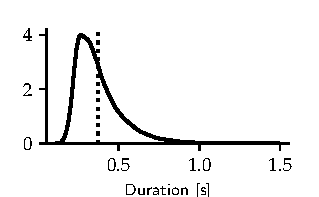
\includegraphics{kick_duration_beamer}

  Overall $64 \times (1 + 2) = 192$ features per timestep
\end{frame}

\begin{frame}
  \frametitle{Social Models---Linear without memory}
  \begin{columns}
   \begin{column}{0.5\textwidth}
  \begin{tikzpicture}[scale=0.5]
   \draw[ultra thick] (0,0)--(0,5);
   \node[rotate=45] at (4.5,4.5) {\textcolor{red}\PHtunny};
   \node[rotate=90] at (2.5,2.5) {\PHtunny};
   \node[rotate=90] at (2.5,0.5) {\textcolor{white}\PHtunny}; % quick hack to align stuff
 \end{tikzpicture}

 \textbf{No memory}: Only current position, etc.
\end{column}~\begin{column}{0.5\textwidth}
\begin{align*}
  \bm{y^i}  &= \bm{X^i_0} \bm{\beta^i_0} + \text{bias} + \varepsilon \\
  \varepsilon &\sim \mathcal{N}\left(0, \sigma^2 \right)
\end{align*}

With:
$\mathcal{N(\text{mean}, \text{variance})}$ normal distribution

$\sigma$ standard deviation of residuals

$\bm{y^i}$ i-th component of output vector

$\bm{X_0^i}, \bm{\beta^i_0}$ input matrix and weights for i-th component and timestep 0
\end{column}
 \end{columns}
  
\end{frame}

\begin{frame}
  \frametitle{Social Models---Linear with memory}
  \begin{columns}
   \begin{column}{0.5\textwidth}
  \begin{tikzpicture}[scale=0.5]
   \draw[red] (3, 3)--(5,5); % our fish
   \draw[ultra thick] (0,0)--(0,5); % wall
   \draw[gray] (2.5, 0)--(2.5,2.5);
   \node[rotate=45] at (4.5,4.5) {\textcolor{red}\PHtunny};
   \node[rotate=90] at (2.5,2.5) {\PHtunny};
   \node[rotate=90] at (2.5,0.5) {\textcolor{gray}\PHtunny};
 \end{tikzpicture}

 \textbf{Memory}: Current position and trace

\end{column}~\begin{column}{0.5\textwidth}
  \textbf{Concatenated}:
  Concatenate features for all timesteps then linear model

  \textbf{Static}:
  Keep spatial weights $\bm{\beta^i_t}$ static for all $t$ 
\begin{equation*}
  \bm{y^i} = \sum_t c_t \bm{X_t^i} \bm{\beta^i} + \varepsilon
\end{equation*}
with $c_t$ mixing coefficient $c_i \geq 0, \sum_i c_i = 1$,
normalized with \textit{softmax}

   \end{column}
 \end{columns}
  
\end{frame}

\begin{frame}
  \frametitle{Social Models---Neural networks}
  \begin{figure}[h]
    \centering
    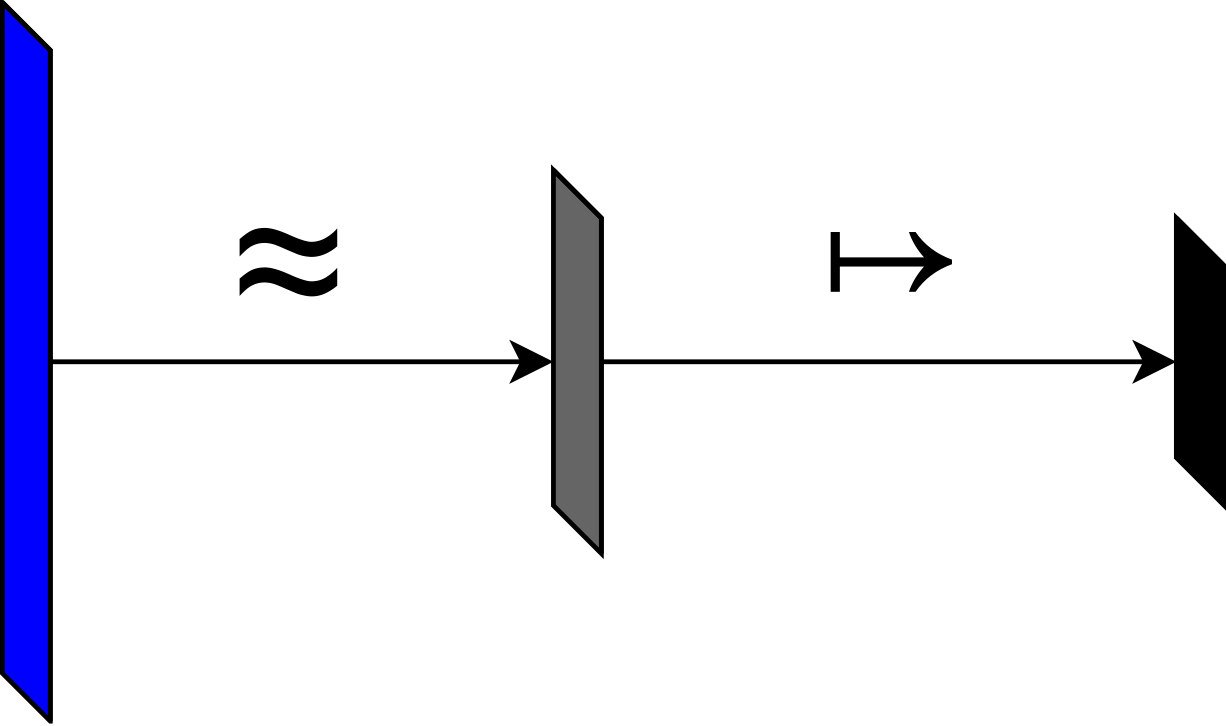
\includegraphics[width=0.45\textwidth]{rf_encoder_decoder}
    \caption*{General architecture.
      Symbols $\approx$ and $\mapsto$ correspond to encoding and decoding. Blue is input, gray hidden and black output.}
  \end{figure}
  \vspace{-0.5cm}
 Neural Networks can capture non-linear effects.

 Encoder-decoder architecture with
 \begin{description}
 \item[Encoder] transforms input features into hidden state
  \item[Decoder] transforms hidden state into output
 \end{description}

 We discuss two encoders \textit{\&} two decoders.
\end{frame}

\begin{frame}
  \frametitle{Neural Networks---Encoders: Multilayer-Perceptron}
  \begin{figure}[h]
    \centering
   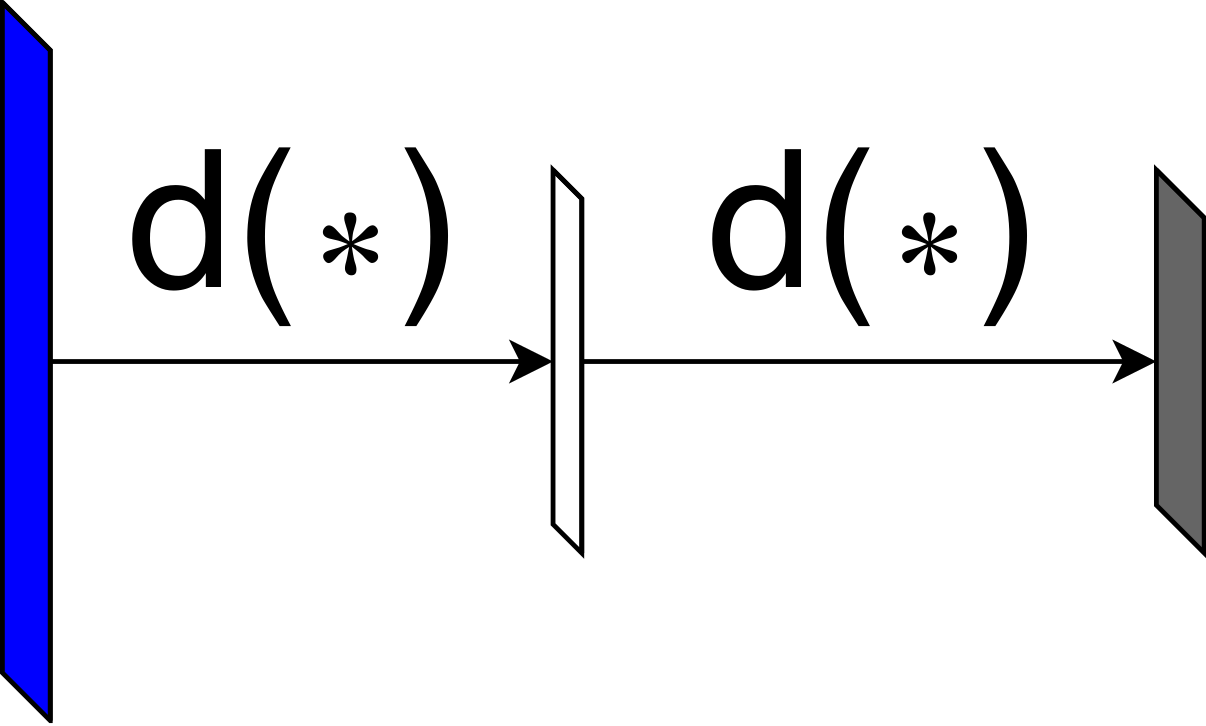
\includegraphics[width=0.45\textwidth]{mlp_encoder} 
   \caption*{%
     Architecture of \textsc{MLP} encoder. Symbol $d(\ast)$ corresponds to linear layer, followed by tanh and dropout~\footfullcite{dropout}.
     Blue is input, gray hidden state.
   }
  \end{figure}
  \vspace{-0.5cm}
    Multilayer perceptron encoder consists of two stacked layers\\(Linear -> Tanh -> Dropout) with 64 hidden neurons.
\end{frame}

\begin{frame}
  \frametitle{Neural Networks---Encoders: Recurrent neural network}
  \begin{figure}[h]
    \centering
   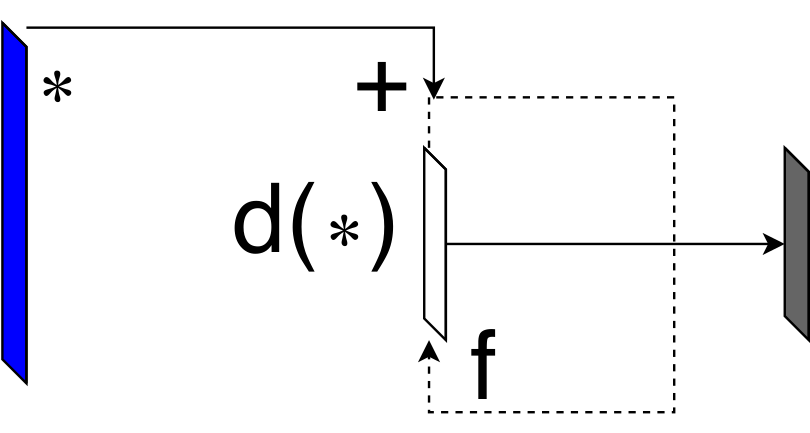
\includegraphics[width=0.45\textwidth]{rnn_encoder} 
   \caption*{%
     Architecture of \textsc{RNN} encoder. Symbol $\ast$ is linear layer, $d(\,)$ is recurrent dropout\footfullcite{recurrentDropout}, $+$ is summation and $f$ to \textit{tanh}.
     Blue is input, gray hidden state.
   }
  \end{figure}
  \vspace{-0.5cm}
Input-to-hidden weights $\bm{w_{ih}}$, hidden-to-hidden weights $\bm{w_{hh}}$, biases $\bm{b}$,
    recurrent dropout $d(\bm{x})$ (same mask for all timesteps), learned initial state of size 64 $(h_0)$
  \begin{equation*}
    \bm{h_t} (\bm{X}) = \operatorname{tanh} \left( \bm{b} + \bm{w_{ih}} \bm{X_t} + \bm{w_{hh}} d (\bm{h_{i-1}}) \right),
  \end{equation*}
\end{frame}

\begin{frame}
  \frametitle{Neural Networks---Decoder: Mixture density networks\footfullcite{mdn}}
  Predict mixture of Gaussians
\begin{equation*}
p \left( \bm{y} | \bm{X} \right) = \sum_{i}^n \kappa_i \mathcal{N} \left( \bm{\mu_i}, \bm{\Sigma_i} \right),
\end{equation*}
with mixing coefficients $\kappa_i$, multivariate normal $\mathcal{N} \left(\bm{\mu_i}, \bm{\Sigma_i}\right)$ with mean vector $\bm{\mu_i}$ and covariance matrix $\bm{\Sigma_i}$
  
Constraints:
$\kappa_i  \geq 0,\, \sum_i \kappa_i = 1$, enforced by \textit{softmax}

$\bm{\Sigma_i}$ valid (diagonal) covariance, diagonals (variances) must be positive, enforced by \textit{exp}.
\end{frame}

\begin{frame}
  \frametitle{Neural Networks---Decoder: Mixture density networks (cont.)\footfullcite{mdn}}
  \begin{figure}[h]
    \centering
    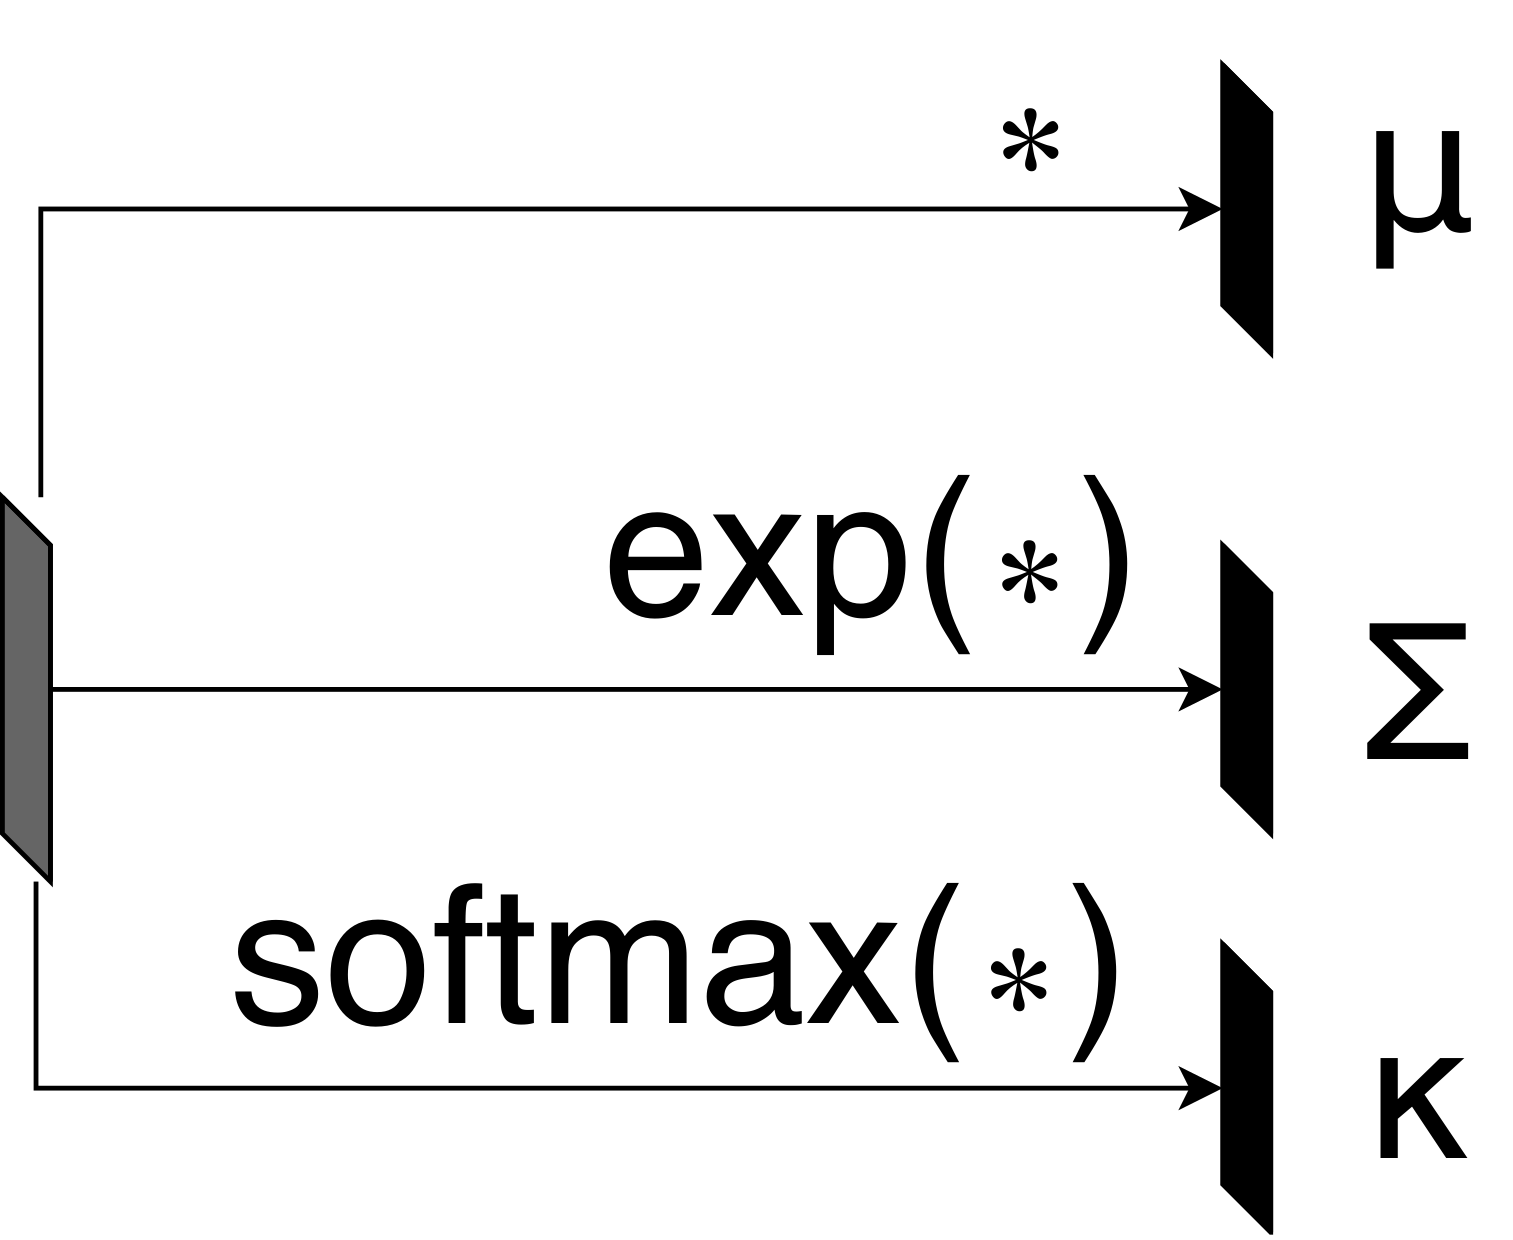
\includegraphics[width=0.45\textwidth]{mdn_decoder}
    \caption*{Architecture of \textsc{MDN} decoder. Symbol $\ast$ is linear layer. Gray is hidden state and black output.}
  \end{figure}

\end{frame}

\begin{frame}
  \frametitle{Results---Quantitative}
\begin{centering}  
\begin{tabular}{@{}lS[table-format=1.2]S[table-format=1.2]S[table-format=1.3]S[table-format=1.3]@{}}
\toprule
{Model} & {\textsc{NLL}-train} & {\textsc{NLL}-test} & {\textsc{MSE}-train} & {\textsc{MSE}-test} \\ \midrule
Baseline (Train-Mean) & 2.25 & 2.01 & 0.558 & 0.423\\
\textsc{MLP-MDN} & 1.63 & \bftabnum 1.60 & 0.448 & 0.373 \\
\textsc{RNN-MDN} & \bftabnum 1.43 & 1.69 & 0.436 & \bftabnum 0.371 \\
\textsc{MLP-MSE} & 2.04 & 1.87 & 0.452 & 0.375 \\
\textsc{RNN-MSE} & 2.00 & 1.86 & \bftabnum 0.432 & 0.377 \\
\midrule
Linear (w/o time) & 2.04 & 1.87 & 0.451 & 0.376 \\
Linear (time conc.) & 2.00 & 1.86 & 0.432 & 0.373 \\
Linear (static spatial) & 2.04 & 1.86 & 0.451 & 0.374 \\
\bottomrule\\
\end{tabular}
\end{centering}
Results for all models. Baseline: Always predict mean.


Note: Comparison of negative log likelihood \textsc{NLL} is valid, all models can be interpreted as mixture of Gaussians.
\end{frame}

\begin{frame}
  \frametitle{Results---Example simulation with \textsc{RNN-MDN}}
\begin{figure}[H]
    \centering
    \movie[width=0.7\textwidth, height=0.7\textwidth, autostart,, loop, poster]{}{social_anim.mp4}
\end{figure}
\end{frame}

\begin{frame}
  \frametitle{Conclusion}
\begin{itemize}
  \item Data-driven discretization leads to more equal fish distribution than standard approach.
  \item Models extend trivially to larger fish groups.
  \item \textsc{MDN}-models allow sampling, multi-modal distributions and model uncertainty.
    This is \alert{biologically more plausible} than our alternatives.
  \item Non-linear models work but do not show a significant improvement (but should work well for larger groups).
\end{itemize}

\end{frame}

%\section{Appendix}
\end{document}